\documentclass{article}
\usepackage{tikz} 
\usepackage[utf8]{inputenc}
\usepackage{amsmath}
\usepackage{listings}
\usepackage{amsfonts}
\usepackage{amssymb}
\usepackage{tabularx}
\usepackage{enumitem}
\usepackage{algorithm}% http://ctan.org/pkg/algorithm
\usepackage[noend]{algpseudocode}% http://ctan.org/pkg/algorithmicx

\usepackage{tikz}

\usepackage{graphicx}
\usetikzlibrary{arrows,positioning} 
\usepackage{subcaption}
\thispagestyle{empty}
\usepackage{multicol,caption}
\pgfarrowsdeclarecombine{ring}{ring}{}{}{o}{o}

\DeclareMathOperator{\ringarrow}{\raisebox{0.5ex}{\tikz[baseline]{\draw[ring->](0,0)--(2em,0);}}}

\tikzset{
    %Define standard arrow tip
    >=stealth',
    %Define style for boxes
    observed/.style={
           circle,
           rounded corners,
           draw=black, thick,
           minimum width=.5em,
           minimum height=.5em,
           font=\footnotesize,
           text centered,
           fill=blue!20!white},
     latent/.style={
           circle,
           rounded corners,
           draw=black, thick, dashed,
           minimum width=.5em,
           minimum height=.5em,
           font=\footnotesize,
           text centered,
           fill=black!10!white
           },
    % Define arrow style
    pil/.style={
           o->,
           thick,
           shorten <=2pt,
           shorten >=2pt,},
    sh/.style={ shade, shading=axis, left color=red, right color=green,
    shading angle=45 }
    
}
   
\begin{document}
\def\ci{\perp\!\!\!\perp} % from Wikipedia


\begin{figure}
\centering
\begin{subfigure}[t]{0.4\textwidth}
\centering
\caption{$(X \ci Y | Z)$}
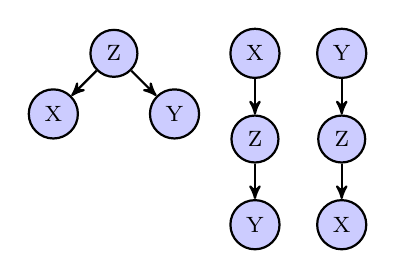
\begin{tikzpicture}[->,shorten >=0pt,shorten <=0pt,node distance=0.45cm,  thick,main node/.style={observed}]
\node[main node](1){Z};
\node[main node, below left=of 1](2){X};
\node[main node, below right=of 1](3){Y};
\path[](1) edge (2) (1) edge (3);
\node[main node, right=of 1,xshift=2em](4){X};
\node[main node, below=of 4](5){Z};
\node[main node, below=of 5](6){Y};
\path[](4) edge (5) (5) edge (6);
	
\node[main node, right=of 4](7){Y};
\node[main node, below=of 7](8){Z};
\node[main node, below=of 8](9){X};
\path[]	(7) edge (8) (8) edge (9);	
\end{tikzpicture}
\end{subfigure}
\begin{subfigure}[t]{0.3\textwidth}
\centering
\caption{v-structure, $(X \ci Y)$}
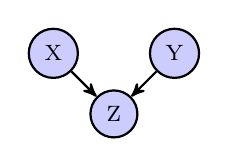
\begin{tikzpicture}[->,shorten >=0pt,shorten <=0pt,node distance=0.45cm,  thick,main node/.style={observed}, shaded/.style={latent}]
\node[main node](1){Z};
\node[main node, above left=of 1](2){X};
\node[main node, above right=of 1](3){Y};
\path[]
    (2) edge (1)
    (3) edge (1); 
\end{tikzpicture}
\end{subfigure}
\end{figure}

\end{document}